\documentclass[conference]{IEEEtran}
\IEEEoverridecommandlockouts
% The preceding line is only needed to identify funding in the first footnote. If that is unneeded, please comment it out.
%Template version as of 6/27/2024

\usepackage{cite}
\usepackage{amsmath,amssymb,amsfonts}
\usepackage{algorithmic}
\usepackage{graphicx}
\usepackage{textcomp}
\usepackage{xcolor}

\usepackage[T1]{fontenc}
\usepackage[utf8]{inputenc}
\usepackage{subcaption}
\usepackage{siunitx}
\usepackage[hidelinks]{hyperref}

\def\BibTeX{{\rm B\kern-.05em{\sc i\kern-.025em b}\kern-.08em
    T\kern-.1667em\lower.7ex\hbox{E}\kern-.125emX}}
\begin{document}

\title{Research Project: Implementation of an In-Memory Key-Value Store Based on Optimized B+ Trees}

\author{\IEEEauthorblockN{Janne Gruhler, Maxim Bellm, Albert Rico Martin, Matthias Raba}
\IEEEauthorblockA{\textit{Department of Computer Science} \\
\textit{Hochschule Furtwangen}\\
Furtwangen, Germany}
}

\maketitle

\begin{abstract}
B\textsuperscript{+}-trees have historically been considered inferior to hash-based structures
for in-memory workloads. Recent work argues that this gap is largely an artifact of
implementation. We converted the reference implementation into a reusable static library
and attempted to reproduce its benchmarks. We also built a Redis-compatible key-value store
and compared it against Redis under YCSB2 Workload~C. Our store becomes competitive beyond
roughly \num{500000} keys and outperforms Redis on range scans. Absolute throughput in our
reproduction deviates from the published values, but qualitative trends are preserved.
\end{abstract}

\begin{IEEEkeywords}
B-Trees, In-Memory Database, Key-Value Store, Memory Layout
\end{IEEEkeywords}

\section{Introduction and Motivation}

B\textsuperscript{+}-trees are among the most fundamental index structures in database
systems, but were long considered inferior for in-memory use. Systems such as Redis rely
on hash-based structures with near-constant latency per access. The paper
\emph{``B-trees are back: Engineering fast and pageable node layouts''} by Müller, Benson
and Leis~\cite{muller2025b} shows this is primarily an implementation artifact: through
multiple node types, fingerprinting, hinting, prefix compression and SIMD acceleration,
B\textsuperscript{+}-trees match or exceed the throughput of the Adaptive Radix Tree~(ART)
and the Height Optimized Trie~(HOT), while preserving key order at no additional cost.
If this holds, the preference for hash-based indexes in in-memory systems is a matter of
implementation history rather than on a structural property, making an ordered index
viable where an unordered one is normally assumed.

\section{Analysis and Setup of the Existing Repository}

The code is publicly available on GitHub but was tightly coupled to one specific compiler
environment: SIMD intrinsics were embedded directly as AVX2 code, the build system was a
hand-written Makefile, and dependencies like TLX had to be placed into the source tree by hand.
In this state the code is difficult to build outside the authors' environment.
We restructured the repository into a static library (\texttt{libbtree}): the build system
was migrated to CMake, the AVX2 intrinsics were moved behind a compiler-independent
abstraction, and the code was updated to compile cleanly under current compilers.
The library exposes a unified \texttt{DataStructureWrapper} interface and can be included
in other projects via CMake. The abstraction, in theory, also allows the code to be compiled for
architectures other than x86, although performance on such systems is untested.

\section{Reproduction of Benchmark Results}

The benchmarks are driven by Python scripts that invoke benchmarking programs with
parameters (key count, operation count, batch size), store results as CSV, and visualize
them in R. Datasets included dense and sparse integer keys, Wikipedia article titles and
randomly generated URLs. All measurements ran on a university VM provisioned with
4~vCPUs and \SI{64}{\giga\byte} of RAM, hosted on an AMD EPYC~7702P. Each core has
\SI{64}{\kibi\byte} of L1 and \SI{512}{\kibi\byte} of L2 cache, alongside
\SI{64}{\mebi\byte} of shared L3; the system runs Debian~13 with kernel~7.0.4.
The benchmark workload is synchronous and single-threaded and therefore executes on one
core; dedicated cores and a single NUMA node rule out contention from co-located tenants.
This setup nevertheless differs from the bare-metal machine of the original publication,
which must be kept in mind when comparing absolute numbers. We compiled with a newer
compiler version but kept the original optimization and architecture flags unchanged.

Reproduction proved considerably more difficult than expected. Datasets are only described
in prose and not included in the repository. Our self-generated substitutes caused reproducible
crashes whose cause could not be determined from the code alone. Not all figures could be
unambiguously attributed to a benchmark script either, so the configuration behind some
published curves remained unclear. After contacting the authors, we received the original
datasets, which resolved the crashes and reduced the discrepancies. Absolute throughput
still deviates from the published values in places by orders of magnitude. We cannot
attribute the remaining gap to a single cause, as differing hardware, a newer toolchain
and possibly different script versions all plausibly contribute. Qualitative trends such as
relative ordering of structures and curve shapes are mostly preserved, as shown
in \autoref{fig:normalized_zipf_minserts} and \autoref{fig:absolute_memory_usage}.

\begin{figure}[htbp]
    \centering
    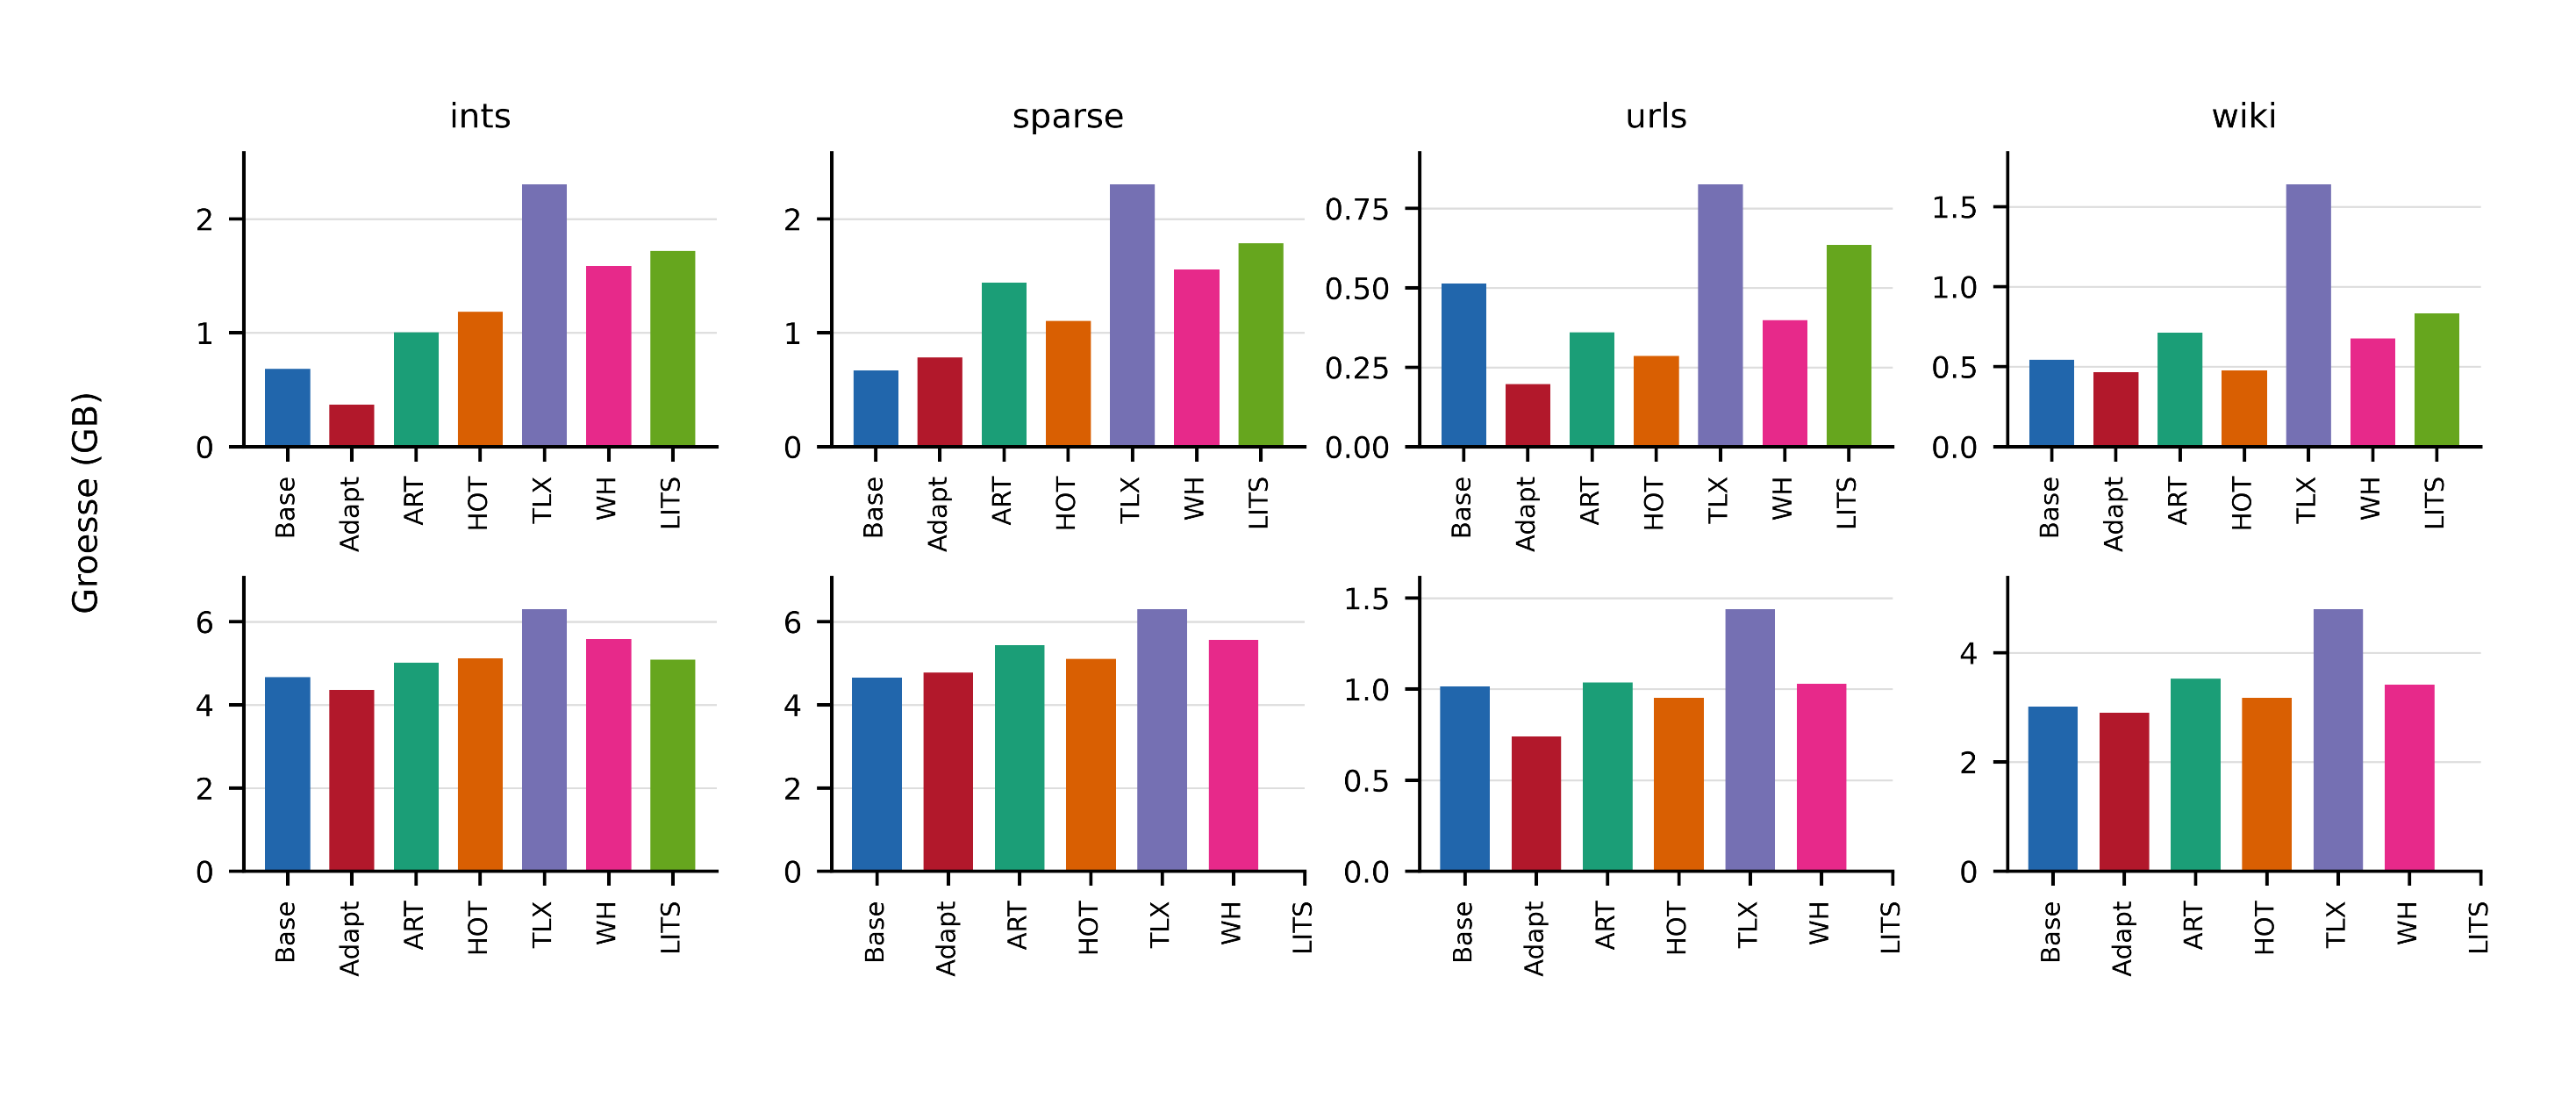
\includegraphics[width=\linewidth]{img/btree_absolute_memory_usage.png}
    \caption{Absolute memory usage. Top: original paper. Bottom: our results.}
    \label{fig:absolute_memory_usage}
\end{figure}

\begin{figure}[htbp]
    \centering
    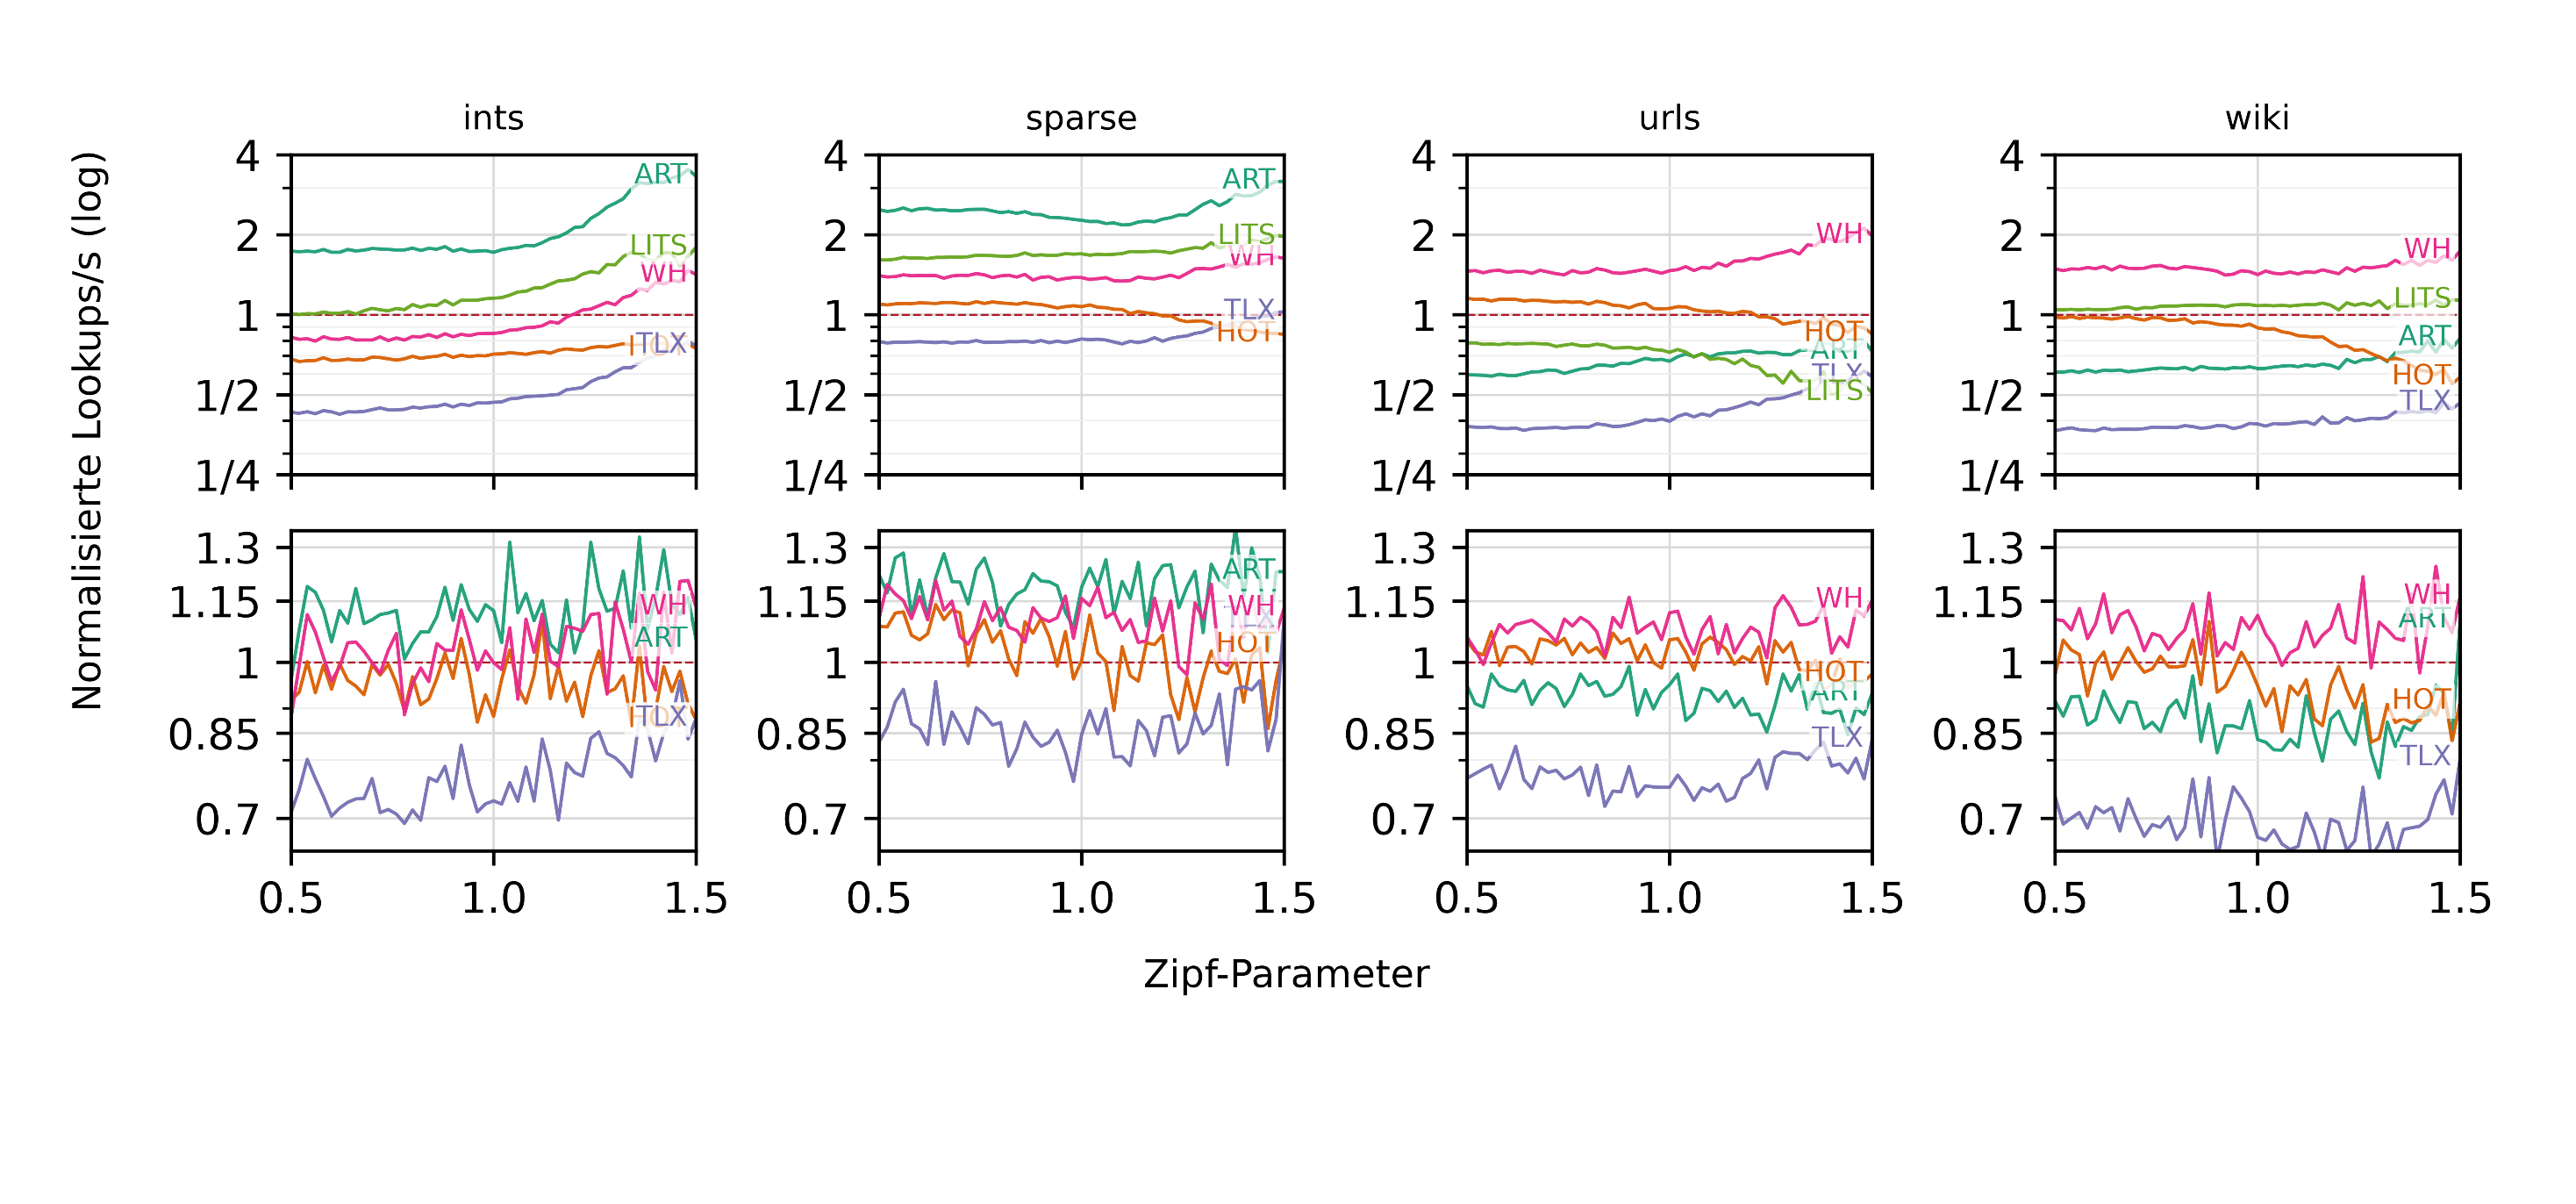
\includegraphics[width=\linewidth]{img/btree_normalized_zipf.png}
    \caption{Minserts normalized to B-Trees. Top: original paper. Bottom: our results.}
    \label{fig:normalized_zipf_minserts}
\end{figure}

\section{Implementation of a Key-Value Store Based on B-Trees}
\label{sec:impl}

Based on \texttt{libbtree}, we built a Redis-compatible key-value store. The first step
was implementing the Redis Serialization Protocol (RESP, Version~2), a text-based encoding
for strings, integers and arrays, sent over TCP via Boost.Asio. The server parses incoming
commands and dispatches them to \texttt{libbtree}. Implemented commands include
\texttt{GET}, \texttt{SET}, \texttt{MGET}, \texttt{MSET}, \texttt{DEL}, \texttt{EXISTS},
\texttt{INCR}/\texttt{DECR}, \texttt{INFO}, and an adaptation of sorted-set operations
(\texttt{ZADD}, \texttt{ZRANGE}). Since the protocol is implemented faithfully, the
resulting server~\cite{btree_redis2026} can be used as a drop-in replacement for Redis.

To compare both systems, YCSB2 was adapted to use a Redis client instead of direct
B-tree operations, so that an identical load can be directed at either server over the
local network. All measurements use Workload~C (100\,\% reads, Zipf-distributed) with
batched \texttt{MGET} and \texttt{MSET} commands of 10\,000 operations each to minimize
network overhead.

\autoref{fig:benchmark-get} shows read throughput by database size. The B-tree store
becomes competitive at around \num{500000} keys. Beyond 2.6~million keys, Redis's
throughput flattens due to O(1) hash lookups while B-tree throughput continues to grow
on an O(log~n) curve.

A structural advantage of B\textsuperscript{+}-trees is their ordered key storage, which
allows range scans without additional data structures. Redis can only provide this through
sorted sets, which maintain a separate index. \autoref{fig:benchmark-range-scan} shows
that with small key counts both systems perform similarly, but Redis's scan duration grows
much more steeply. At around 3~million keys, Redis scans take roughly twice as long, and
this gap does not close as the database grows further.

\begin{figure}[htbp]
    \centering
    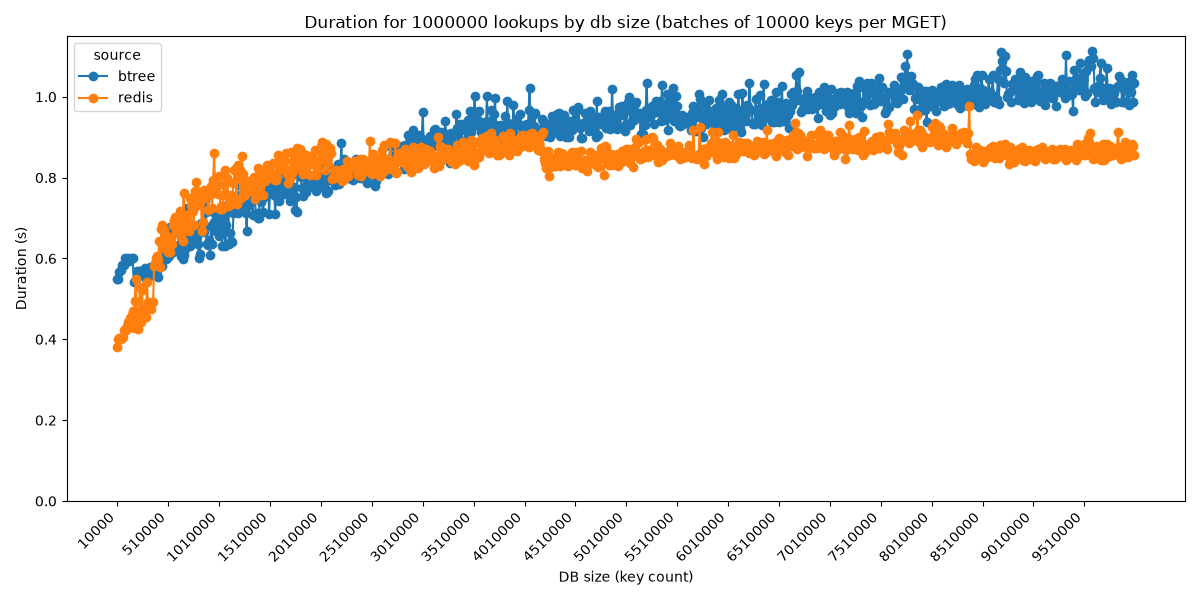
\includegraphics[width=\linewidth]{img/redis_get_benchmark}
    \caption{YCSB2 Workload~C: Throughput B-Tree vs.\ Redis by database size.}
    \label{fig:benchmark-get}
\end{figure}

\begin{figure}[htbp]
    \centering
    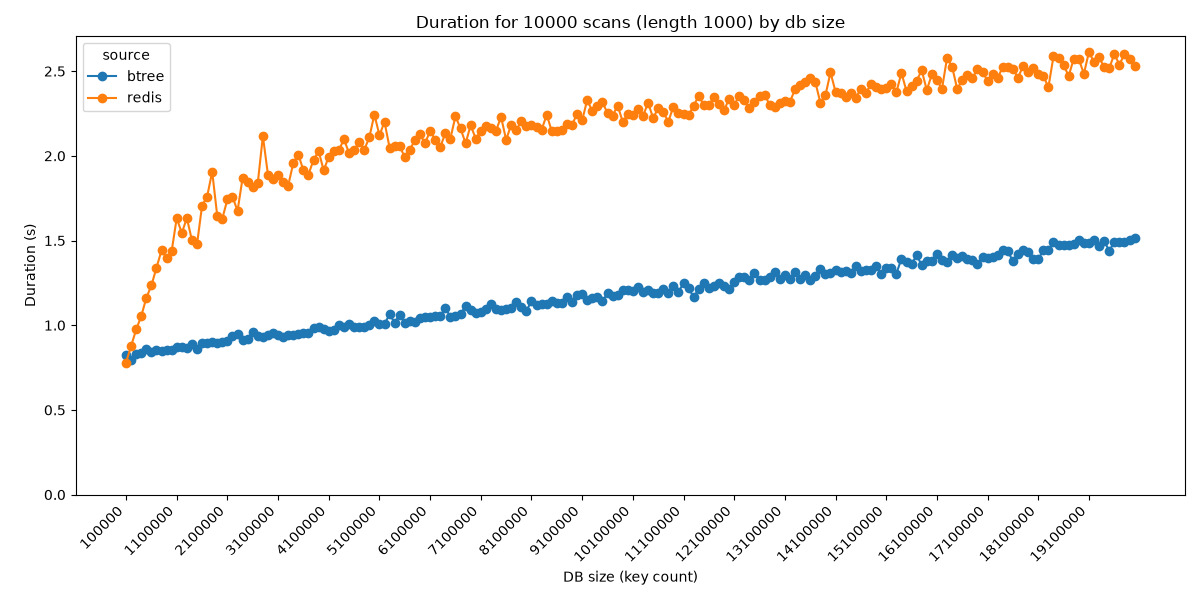
\includegraphics[width=\linewidth]{img/redis_range_scan_benchmark}
    \caption{Throughput of range scans: B-Tree vs.\ Redis by database size.}
    \label{fig:benchmark-range-scan}
\end{figure}

\section{Conclusion}

Optimized B\textsuperscript{+}-trees are a solid foundation for competitive in-memory
key-value stores. Our Redis-compatible implementation confirms this: it reaches competitive
read throughput on sufficiently large datasets, and its ordered key storage gives it a
structural advantage on range scans that a hash-based store can only match by maintaining
an additional index.

The reproduction was the more instructive part of the project. The published code alone
is not sufficient for reproducing the benchmarking results. The datasets, the machine
configuration and an unambiguous mapping from figures to scripts were needed as well, and
only the first of these could be recovered, by contacting the authors directly. In a field
where performance claims are the primary contribution, experimental artifacts deserve the
same care in publication as the source code.

\nocite{*}
\bibliographystyle{IEEEtran}
\bibliography{sources}

\end{document}